\documentclass{myproject}

\graphicspath{{../Figures/}}

% title setup
\title{\vspace*{-1cm}Solution to the Inviscid Burgers' Equation by the Lax-Friedrichs Scheme\footnote{Placeholder title!}}
\date{}
\author{
    Andre Gormann\\
    agormann@sfu.ca
    \and
    Ethan MacDonald\\
    jem21@sfu.ca
}

% bibliography
\addbibresource{references.bib}

\renewcommand*{\thefootnote}{[\arabic{footnote}]}

\begin{document}

% title creation
\maketitle
\vspace*{-1cm}

% document 

\section{Introduction}

The problem we will be considering is the Inviscid Burgers' equation with periodic boundary conditions
\begin{equation}
    \begin{cases}
        & u_t + uu_x = 0 \qquad x \in [-L, L] \qquad t \geq 0 \\
        & u(x,0) = u_0(x) \\
        & u(-L,t) = u(L,t)
    \end{cases}
\end{equation}

Throughout the ensuing discussion, it will be far more useful if we rewrite the Inviscid Burgers' equation in its conservation form
\begin{equation}
    u_t + f(u)_x = 0 \qquad f(u) = \frac{1}{2}u^2
\end{equation}

We have chosen to use the Lax-Friedrichs scheme to approximate solutions of the Inviscid Burgers equation. The scheme is defined by the update rule

\[
    U_j^{n+1} = \frac{1}{2}\left( U_{j-1}^{n} + U_{j+1}^{n} \right) - \frac{\Delta t}{2\Delta x}\left( f(U_{j+1}^{n}) - f(U_{j-1}^{n}) \right)
\]
where $U_{j}^{n} \in \R^N$ denotes the approximation to $u(x_j,t_n)$ at time $t_n$

The scheme combines updates in the spacial domain with time-stepping. Our reasoning for choosing the Lax-Friedrichs scheme is found in the second term of the update rule. This term applies a sort of dampening effect at each time-step based on the flow between grid cells. Specifically, we are effectively modeling the advection-diffusion equation
\[
    u_t + f(u)_x = \frac{(\Delta x)^2}{2\Delta t}u_{xx},
\]
and so are introducing a form of `numerical viscosity.' The reason why this is not problematic is that as the grid is refined, the coefficient in front of $u_{xx}$ vanishes. We hope that this will work to improve accuracy around shocks when they form in the solution. Another advantage of the Lax-Friedrichs scheme is that we can guarantee stability through the choices of ${\Delta t}$ and ${\Delta x}$, so long as we can bound $|u|$. This will be elaborated upon later in the document. We will be testing grid sizes of decreasing powers of $10$, starting with $10^{-1}$. Our choice of ${\Delta t}$ such that stability is guaranteed will therefore depend on the grid size. We will be using periodic boundary conditions because the Inviscid Burgers' equation deals with wave propagation.

\section{Theory}
\subsection{Conservation Laws}
We will begin by introducing notation and then move on to discussion about the theory. First we discretize the interval $[-L,L]$ into a vector of $N$ points $x_j$ by defining a mesh width $\Delta x = 2L/N$ so that 
\[
    x_j = -L + j\Delta x.
\]
Note that we are assuming periodic boundary conditions so that $x_0 = x_{N}$, and so we have exactly $N$ points. For reasons that will soon become clear, we are also interested in the half-steps $x_{j\pm1/2}$ defined by
\[
    x_{j\pm1/2} = x_j \pm \frac{\Delta x}{2}.
\]

We will also denote the time step by $\Delta t_n$ so that
\[
    t_n = n\Delta t_n.
\]
The exact formula for $\Delta t_n$ will remain undefined for now as it must be a variable time-step.

We denote the \emph{pointwise values} of the true solution at the mesh point $(x_j, t_n)$ by 
\[
    u_j^n = u(x_j,t_n).
\]
For finite difference methods, at each time step $t_n$ we are computing a vector $U^n \in \R^N$ where the $j$-th component $U_j^n$ approximates the true solution $u_j^n$. Specifically for conservation laws though, it is perhaps more natural to instead view $U_j^n$ as approximating the \emph{cell average} $\bar{u}_j^n$ (see Figure 1) about the mesh point $(x_j,t_n)$ where
\begin{equation}
    \bar{u}_j^n = \frac{1}{\Delta x} \int_{x_{j-1/2}}^{x_{j+1/2}} u(x,t_n) dx.
\end{equation}
The motivation for this interpretation comes from the integral form of the conservation law\footnote{Interestingly, we are somewhat doing things backwards. The conservation law is derived from the integral form, and the PDE that satisfies it is a consequence of this integral form.} (2),
\[
    \frac{d}{dt} \int_{x_j-1/2}^{x_j+1/2} u(x,t)dx - \left[ f(u(x_{j-1/2},t)) - f(u(x_{j+1/2},t)) \right] = 0,
\]
for which a derivation can be found in \cite{leveque1992}, pp. 14-16. Integrating from $t_n$ to $t_{n+1}$ yields
\begin{align*}
    \int_{x_{j-1/2}}^{x_{j+1/2}} u(x,t_{n+1}) dx = &\int_{x_{j-1/2}}^{x_{j+1/2}} u(x,t_{n}) dx \\
    &- \left[ \int_{t_n}^{t_{n+1}} f(u(x_{j+1/2},t)) dx - \int_{t_n}^{t_{n+1}} f(u(x_{j-1/2},t)) dx \right].
\end{align*}
Now dividing by $\Delta x$ and using the definition of (3) results in
\begin{equation}
    \bar{u}_j^{n+1} = \bar{u}_j^n - \frac{1}{\Delta x}\left[ \int_{t_n}^{t_{n+1}} f(u(x_{j+1/2},t)) dx - \int_{t_n}^{t_{n+1}} f(u(x_{j-1/2},t)) dx \right].
\end{equation}

\begin{figure}[h]
    \centering
    \begin{subfigure}[b]{0.8\textwidth}
        \centering
        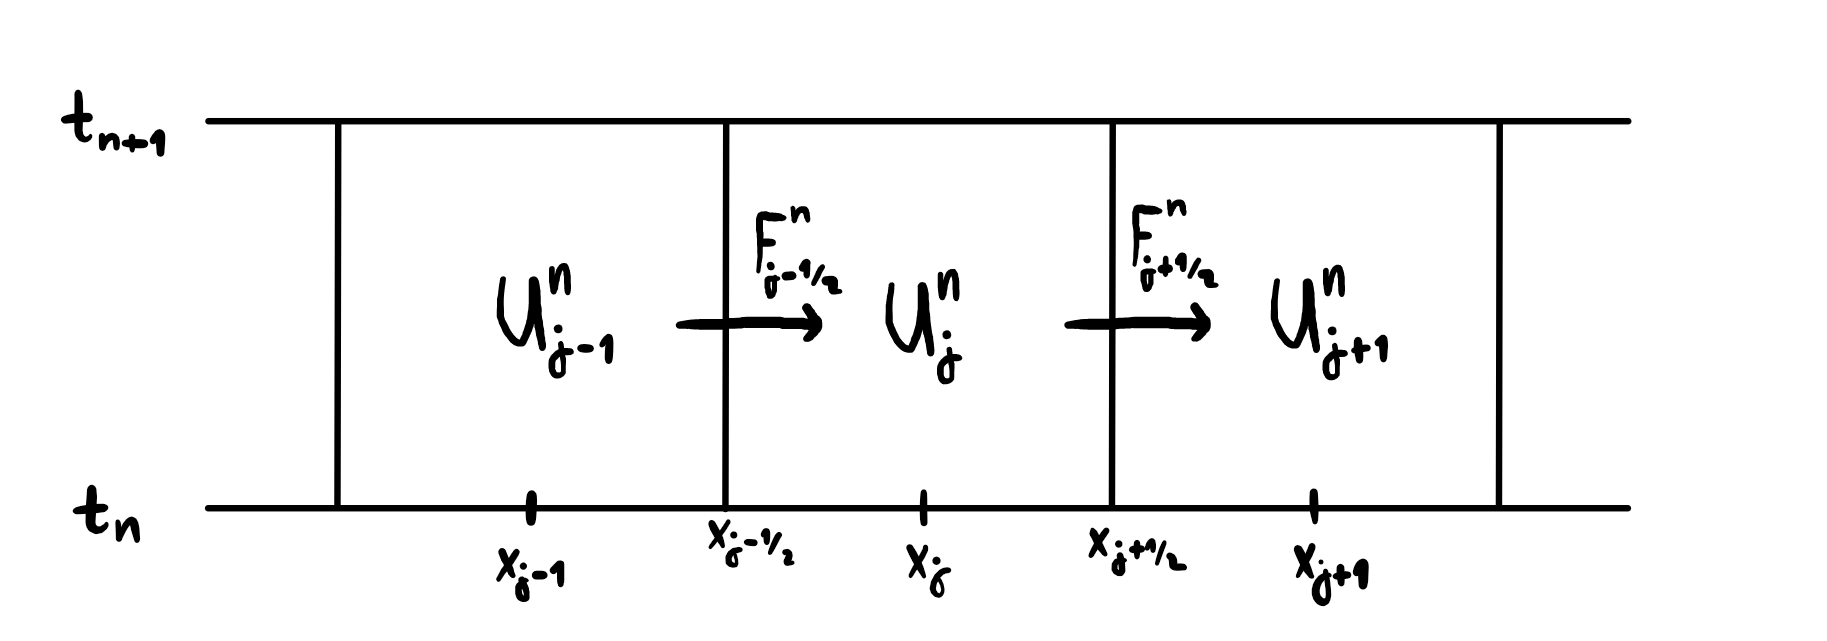
\includegraphics[width=0.90\textwidth]{control_volumes.png}
        \caption{Illustration of the cell averages. Inspired from Fig 4.1, p.65 of \cite{leveque2002}.}
    \end{subfigure}

    \vspace{\floatsep}

    \begin{subfigure}{0.8\textwidth}
        \centering
        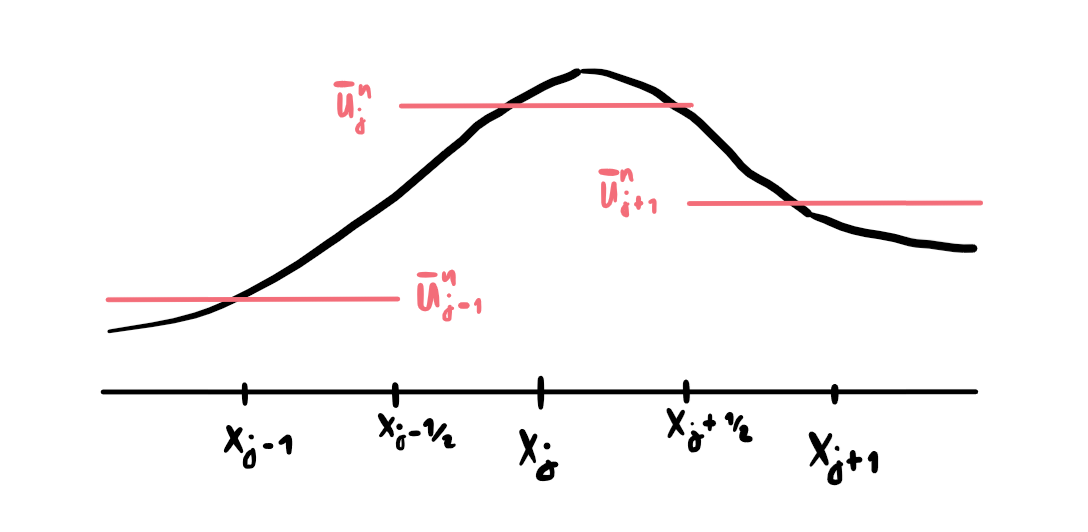
\includegraphics[width=0.90\textwidth]{step-wise_approx.png}
        \caption{Illustration of the step-wise nature the cell-average approximation to $u(x_j,t_n)$ has. Inspired from Fig 17.9, p.418 of \cite{iserles2009}.}
    \end{subfigure}
    \caption{}
\end{figure}

The goal of a successful numerical scheme then is to accurately model the flux through the boundaries of each cell. Explicitly, we want to find some numerical flux function $\mathcal{F}$ so that 
\[
    \mathcal{F}(U_j^n, U_{j+1}^n) \approx \frac{1}{\Delta t} \int_{t_n}^{t_{n+1}} f(u(x_{j+1/2}, t)) dt \qquad \mathcal{F}(U_{j-1}^n, U_{j}^n) \approx \frac{1}{\Delta t} \int_{t_n}^{t_{n+1}} f(u(x_{j-1/2}, t)) dt.
\]

To this end, we say that a numerical method is in \emph{conservation form} if 
\[
    U_j^{n+1} = U_j^n - \frac{\Delta t}{\Delta x} \left[ \mathcal{F}(U_{j}^{n}, U_{j+1}^{n}) - \mathcal{F}(U_{j-1}^{n}, U_{j}^{n}) \right].
\]
Note that while this derivation comes about through the introduction of control volumes, and hence falls under the umbrella of \emph{finite volume methods}, we can also understand it through the lens of finite differences. Specifically, from (2) we get the relation
\[
    \frac{U_j^{n+1} - U_j^n}{\Delta t} + \frac{F_{j+1/2}^n - F_{j-1/2}^n}{\Delta x} = 0
\]
where $F_{j\pm1/2}^n \sim \mathcal{F}$ as before. Hence these methods can be understood to be first-order accurate in time and `somewhat' second-order accurate in space. We say `somewhat' because the reality is complicated.

\subsection{Convergence}
To ensure a numerical scheme converges to the correct solution, we impose a few restrictions on the construction of the numerical flux function $\mathcal{F}$. First, we require that it is \emph{Lipschitz continuous}. That is, when $u(x_j,t_n) \approx \bar{u}_j^n$ about some mesh point $(x_j,t_n)$, that we can find $M \in \R$ so that
\begin{equation}
    \left| \mathcal{F}(U_{j-1}^n, U_j^n) - f(\bar{u_j^n}) \right| \leq M \max\left( \left| U_j^n - \bar{u^n_j} \right|, \left| U_{j-1}^n - \bar{u_j^n} \right| \right).
\end{equation}
The condition for stability is dependent upon the method employed. Since we will be using Lax-Friedrichs, we require that as the step-sizes $\Delta x$ and $\Delta t$ are refined, that the following inequality is maintained
\begin{equation}
    \max_{j \in [1, N]} |U_j^n| \frac{\Delta t}{\Delta x} \leq 1
\end{equation}

We mentioned prior that the time-step $\Delta t$ must be variable. The reason for this will now be illustrated (see Figure 2 below). The entire reason for the cell-average interpretation is so that we can chop the interval into a collection of Riemann problems. If we have shockwaves (or rarefactions) interacting with one another, the problem is no longer a Riemann problem and the method breaks down. Hence the time-step must be catered to the problem.
\begin{figure}[h]
    \centering
    \begin{subfigure}[b]{0.49\textwidth}
        \centering
        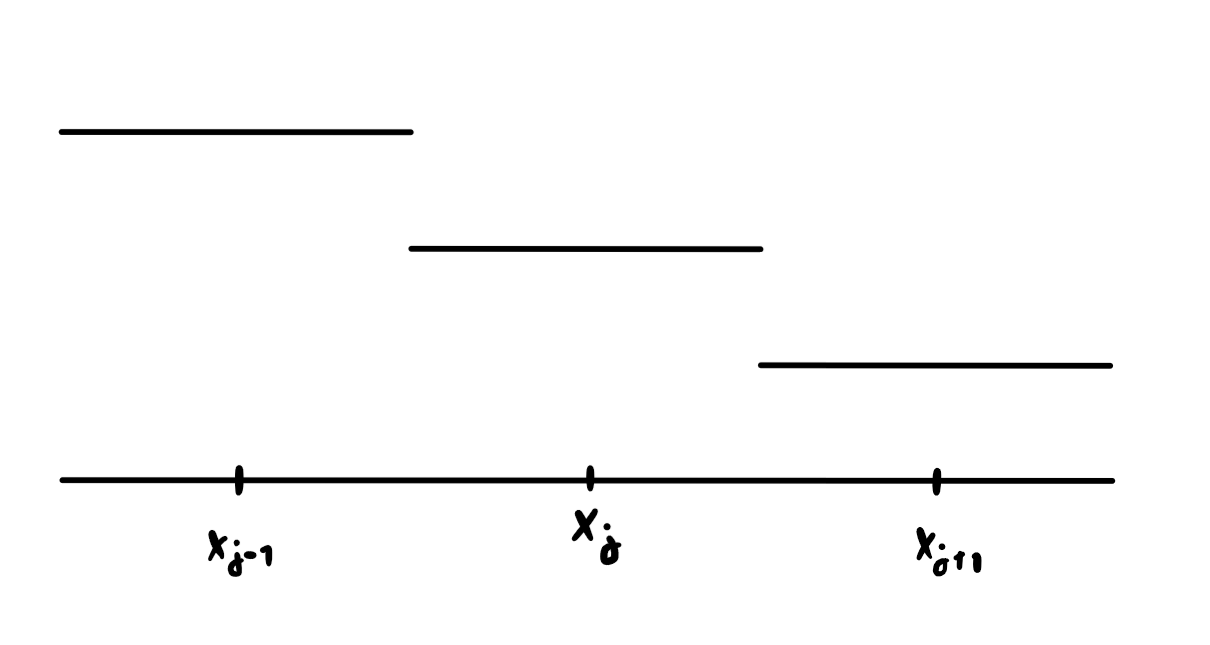
\includegraphics[width=\textwidth]{steps_for_shocks_crossing_cells.png}
        \caption{Cell averages of some toy function. Notice that by the Rankine–Hugoniot conditions, we expect shockwaves to propagate at the discontinuities.}
    \end{subfigure}\hfill
    \begin{subfigure}{0.49\textwidth}
        \centering
        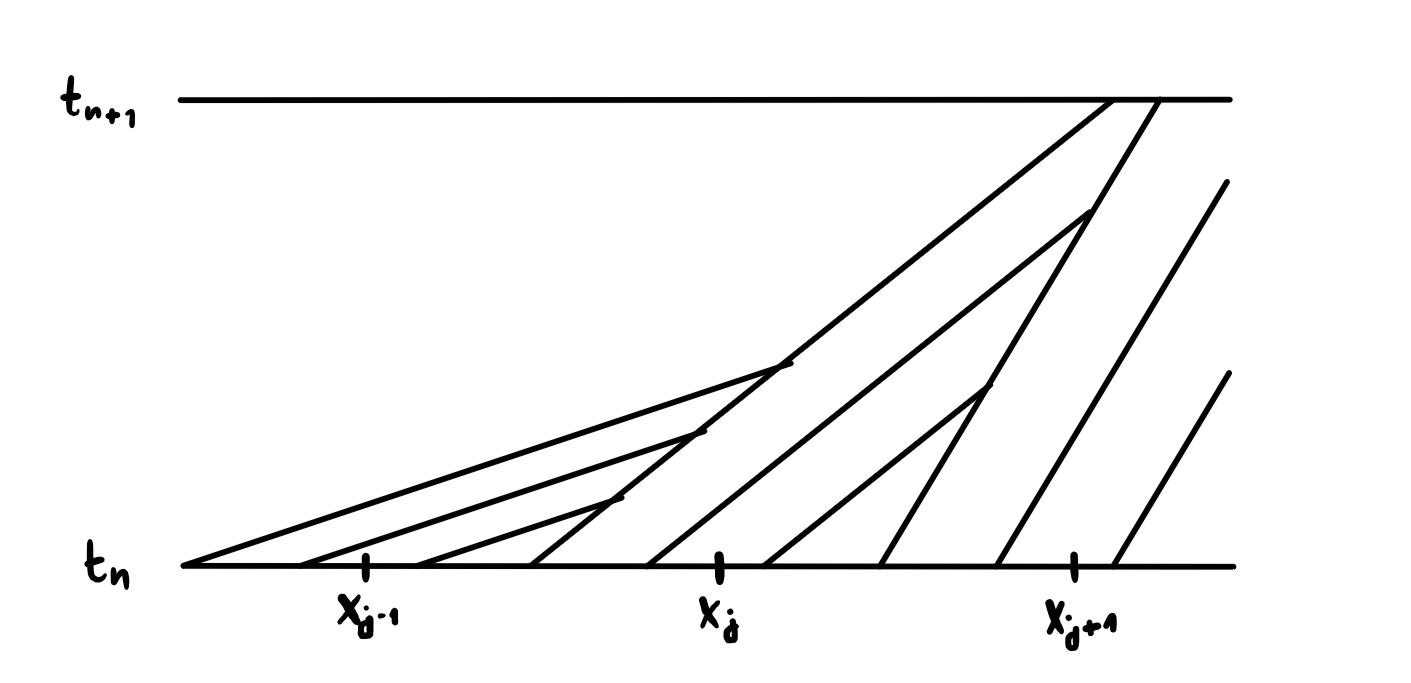
\includegraphics[width=\textwidth]{shockwaves_crossing_multiple_cells.png}
        \caption{Characteristic curves associated with the cell averages. Notice that the shockwave from the first discontinuity is carried into the third cell because the time-step $\Delta t$ is too large.}
    \end{subfigure}
    \caption{}
\end{figure}

As an aside: the unfortunate reality\footnote{At least, this is our current comprehension. The theory is somewhat overwhelming and hard to understand.} is that the aforementioned conditions are insufficient for guaranteeing convergence. We also require that the method satisfies the Lax-Wendroff Theorem. We will not state it here because we do not fully comprehend it, but it can be found on page 130 of \cite{leveque1992} and page 240 of \cite{leveque2002}. Further, we require that the method satisfies a certain \emph{entropy condition}. \cite{iserles2009} on page 416 states it simply as the inequality
\[
    1/2 uu_t + 1/3 u^2u_x \leq 0
\]
but the discussion on pages 133-135 of \cite{leveque1992} and pages 243-244 of \cite{leveque2002} seem to imply it is more complicated than that. The consequence of satisfying this condition is quite important, as it appears that it guarantees that the method correctly and accurately models shockwaves and rarefactions.

\section{Matrix Form of the Lax-Friedrichs Scheme}
The Lax-Friedrichs scheme
\[
    U_j^{n+1} = \frac{1}{2}\left( U_{j-1}^{n} + U_{j+1}^{n} \right) - \frac{\Delta t}{2\Delta x}\left( f(U_{j+1}^{n}) - f(U_{j-1}^{n}) \right)
\]

can be converted into a matrix form

\[
\vec{U}^{n+1} = A\vec{U}^{n} - B\vec{f}(\vec{U}^{n})
\]

where

\[
A = \frac{1}{2}
\begin{bmatrix}
0 & 1 & 0 & \dots & 0 & 1 \\
1 & 0 & 1 & \dots & 0 & 0 \\
0 & 1 & 0 & \dots & 0 & 0 \\
\vdots & \vdots & \vdots & \ddots & \vdots & \vdots \\
0 & 0 & 0 & \dots & 0 & 1 \\
1 & 0 & 0 & \dots & 1 & 0
\end{bmatrix},
\quad
B = \frac{\Delta t}{2 \Delta x}
\begin{bmatrix}
0 & 1 & 0 & \dots & 0 & -1 \\
-1 & 0 & 1 & \dots & 0 & 0 \\
0 & -1 & 0 & \dots & 0 & 0 \\
\vdots & \vdots & \vdots & \ddots & \vdots & \vdots \\
0 & 0 & 0 & \dots & 0 & 1 \\
1 & 0 & 0 & \dots & -1 & 0
\end{bmatrix}
\]

If we instead use the conservation form of the Lax-Friedrichs scheme

\[
    U_j^{n+1} = U_j^n - \frac{\Delta t}{\Delta x} \left( \mathcal{F}(U_{j}^{n}, U_{j+1}^{n}) - \mathcal{F}(U_{j-1}^{n}, U_{j}^{n}) \right)
\]

\[
    \mathcal{F}(U_j^n, U_{j+1}^n) := \frac{\Delta x}{2 \Delta t}(U_j^n - U_{j+1}^n) + \frac{1}{2}\left( f(U_j^n) + f(U_{j+1}^n) \right)
\]

we get the following matrix form

\[
\vec{U}^{n+1} = \vec{U}^{n} - C\vec{\mathcal{F}}(\vec{U}^{n})
\]

\[
\vec{\mathcal{F}}(\vec{U}^{n}) = D\vec{U}^{n} + E\vec{f}(\vec{U}^{n})
\]

where

\[
C = \frac{\Delta x}{\Delta t}
\begin{bmatrix}
-1 & 1 & 0 & \dots & 0 & 0 \\
0 & -1 & 1 & \dots & 0 & 0 \\
0 & 0 & -1 & \dots & 0 & 0 \\
\vdots & \vdots & \vdots & \ddots & \vdots & \vdots \\
0 & 0 & 0 & \dots & -1 & 1 \\
1 & 0 & 0 & \dots & 0 & -1
\end{bmatrix},
\]
\[
D = \frac{\Delta x}{2 \Delta t}
\begin{bmatrix}
-1 & 0 & 0 & \dots & 0 & 1 \\
1 & -1 & 0 & \dots & 0 & 0 \\
0 & 1 & -1 & \dots & 0 & 0 \\
\vdots & \vdots & \vdots & \ddots & \vdots & \vdots \\
0 & 0 & 0 & \dots & -1 & 0 \\
0 & 0 & 0 & \dots & 1 & -1
\end{bmatrix},
\quad
E = \frac{1}{2}
\begin{bmatrix}
1 & 0 & 0 & \dots & 0 & 1 \\
1 & 1 & 0 & \dots & 0 & 0 \\
0 & 1 & 1 & \dots & 0 & 0 \\
\vdots & \vdots & \vdots & \ddots & \vdots & \vdots \\
0 & 0 & 0 & \dots & 1 & 0 \\
0 & 0 & 0 & \dots & 1 & 1
\end{bmatrix}
\]

In either case, we can construct the matrices in MATLAB by using the \texttt{diag()} command on vectors containing the values of the non-zero diagonals, then filling in the values in the bottom left and top right corners as necessary, and lastly multiplying by the respective coefficient.

We will be using the matrices defined in this section to implement our periodic boundary conditions. The entries in the bottom left and top right corners of the matrices handle the cases where a value from beyond the periodic boundaries is needed.

\section{Conclusion}

The primary numerical scheme we hope to implement and study will be the Lax-Friedrichs scheme, for the reasons already stated. This does not preclude us from considering other methods though. Specifically, we have been looking at the Richtymer two-step Lax-Wendroff method and several variations of the Godunov method. The reason for the modified Lax-Wendroff method is that the Lax-Friedrichs method is only first-order accurate in space (so is the unmodified Godunov method). While the two-step modification allows Lax-Wendroff to be second-order accurate, oscillations are introduced as a result and hence it is not entirely satisfactory. There are of course solutions to these problems in the form of `flux limiters' and `total variation diminishing' methods (which appear to use the Godunov method as a `base'). The theory is a lot more complicated though, and so we plan to continue research.

% bibliography
% \nocite{choksi2022}
\nocite{iserles2009}
% \nocite{kutz2013}
% \nocite{trefethen2000}
% \nocite{learncfd}
% \nocite{evans2010}
\nocite{leveque1992}
\nocite{leveque2002}
\printbibliography

\end{document}